\documentclass{beamer}
\usetheme{Berlin}

\usepackage{threeparttable}
\usepackage{graphicx}
\usepackage{booktabs}
\usepackage{makecell}
\usepackage{blkarray}
\setbeamertemplate{navigation symbols}{}

% Author, Title, Date
\title[Fundamental Momentum]{Fundamental Momentum Based Stock Investing}
\author[]{Sicheng~Wang\and Taoying~Zhao\and Pengcheng~Zhou\\~\\
Advisor: Rob Reider,~Method Investment \& Advisory Ltd}
\centering
\date{Capstone Project, 2024}
% Table of Contents
\AtBeginSection[]
{
	\begin{frame}
		\frametitle{Table of Contents}
		\tableofcontents[currentsection]
	\end{frame}
}
% Document
\begin{document}
    \maketitle
    \begin{frame}
        \frametitle{Table of Contents}
        \tableofcontents
    \end{frame}

% Section 1: Introduction
\section{Introduction}
\begin{frame}
    \frametitle{Background}
    \begin{block}{Extensive Research on Momentum Strategies}
        \begin{itemize}
            \item Explaining the profitability of momentum strategies {\color{blue} (Chan et al., 1996)}
            \item Exploring the effectiveness of momentum strategies across diverse asset classes {\color{blue} (Asness et al., 2013)}
            \item Constructing momentum factor to describe the cross-sectional variation of commodity returns {\color{blue} (Bakshi et al., 2019)}
        \end{itemize}
    \end{block}
\end{frame}

\begin{frame}
    \frametitle{Motivation}
    \begin{block}{Recent Development in Momentum Strategies}
        \begin{itemize}
            \item The traditional momentum is based on prices (i.e. {\bf price momentum}).
            \item {\bf Basis-momentum} factor proposed by {\color{blue} Boons and Prado (2019)} shows effective performance on predicting commodity premiums in
            both the time series and cross-section.
            \item {\bf Macro momentum} strategies developed by {\color{blue} Brooks (2017)} demonstrates consistent performance over a half-century.
            \item {\bf Fundamental momentum} strategy proposed by {\color{blue} Novy-Marx (2015)} provides more stable and significant performance compared with price momentum.
        \end{itemize}
    \end{block}
\end{frame}

\begin{frame}
    \frametitle{Main Results}
    \begin{block}{Goal of Our Project}
        {\color{blue} Novy-Marx (2015)} looks at one form of fundamental momentum, earnings per share momentum, 
        whereas we mainly focus on another form of fundamental momentum, profit margin momentum, so that we can provide a better understanding of the momentum profile.
    \end{block}
    \begin{block}{Empirical Interests}
        \begin{itemize}
            \item Strategy performance in back-testing framework.
            \item Spanning tests.
            \item Relation with traditional price momentum strategies.
            \item Conditional strategies.
        \end{itemize}
    \end{block}
\end{frame}

% Section 2: Data and Methodology
\section{Data and Methodology}
\begin{frame}
    \frametitle{Data}
    \begin{block}{Data Sources: WRDS}
        \begin{itemize}
            \item {\bf Monthly Stock Data:} CRSP database.
            \item {\bf Quarterly Company Data:} Compustat database.
        \end{itemize}
    \end{block}
    \begin{block}{Data Process}
        \begin{itemize}
            \item {\bf Time Range:} from January 1975 to December 2023.
            \item Use CUSIP to match the stock price with the fundamental data (24260 stocks in the panel).
            \item Negative prices are dropped.
        \end{itemize}
    \end{block}
\end{frame}

\begin{frame}
    \frametitle{Methodology: Backtesting Framework}
    \begin{block}{Quarterly-rebalanced Sorted Portfolio}
        \begin{itemize}
            \item At each March, June, September, and December, we construct 10 sorted (equally-weighted) portfolios based on the selected fundamental momentum and hold for 3 months.
            \item If the momentum data is missing when we rebalance the portfolio, we use the most recent data up to two months.
            \item Considering the liquidity, we exclude the stocks with the lowest 30\% volume.
            \item Transaction costs: 20 basis for long-only portfolio and 40 basis for long-short portfolios when rebalancing. (a rough but relatively conservative estimate based on \textcolor{blue}{Frazzini, Israel, and Moskowitz (2015)})
        \end{itemize}
    \end{block}
\end{frame}

\begin{frame}
    \frametitle{Methodology: Profit Margin Momentum}
    \begin{block}{Why Profit Margin?}
        \begin{itemize}
            \item Profit margin (PM) is a financial metric that indicates how much of a company's revenue remains as profit after covering all expenses.
            \begin{equation}
                PM = \frac{Net~Income}{Revenue}
            \end{equation}
            \item A higher profit margin indicates a more profitable company that has better control over its costs compared to its competitors.
        \end{itemize}
    \end{block}
\end{frame}

\begin{frame}
    \frametitle{Methodology: Profit Margin Momentum}
    \begin{block}{Factor Construction}
        \begin{equation}
            \text{PM Momentum}(t) = \frac{PM(t) - PM(t-3)}{SD(PM_{Last~3Yrs})}
        \end{equation}
        \begin{itemize}
            \item To increase the stability, we standardize the profit margin momentum by the standard deviation of the profit margin over the last 3 years.
            \item Moreover, we require that there are at least 6 observations in the last 3 years to calculate the standard deviation.
        \end{itemize}
    \end{block}
\end{frame}

% Section 3: Empirical Results
\section{Empirical Results}
\begin{frame}
    \frametitle{Sorted Portfolio based on Profit Margin Momentum}
    \begin{figure}
        \centering
        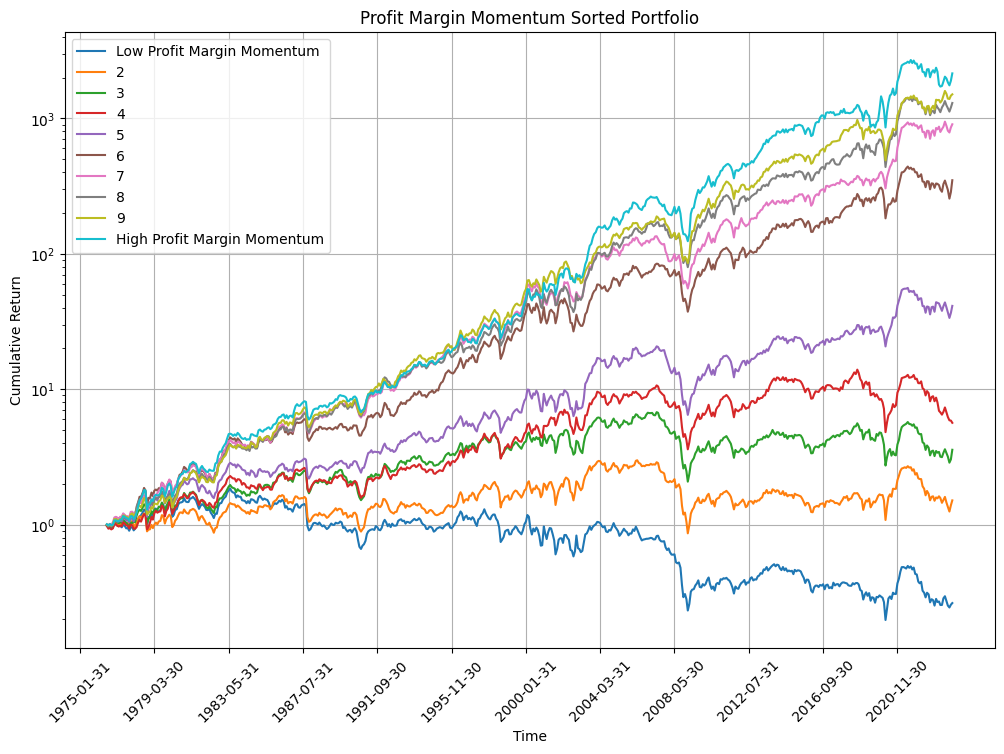
\includegraphics[width=.80\textwidth]{Images/pm_sort.png}
    \end{figure}
\end{frame}

\begin{frame}
    \frametitle{Long-short Portfolio based on Profit Margin Momentum}
    \begin{minipage}[c]{0.6\textwidth}
        \centering
        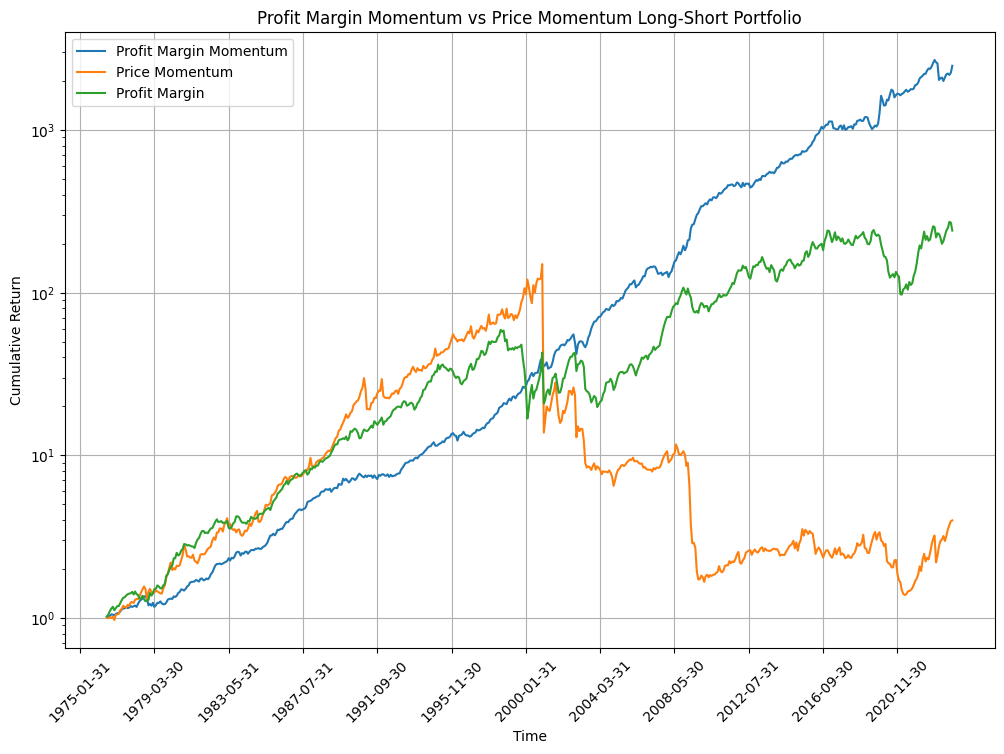
\includegraphics[width=\textwidth]{Images/pm_ls.png}
    \end{minipage}
    \hspace{0.01\textwidth} 
    \begin{minipage}[c]{0.3\textwidth}
        \centering
        \scalebox{0.4}{
\begin{tabular}{llll}
\toprule
 & PM Momentum & Price Momentum & PM \\
\midrule
Mean & 17.34\% & 9.58\% & 14.06\% \\
Std & 12.55\% & 29.27\% & 22.48\% \\
SR & 1.38 & 0.33 & 0.63 \\
MDD & 25.70\% & 99.07\% & 71.53\% \\
\bottomrule
\end{tabular}
        }
    \end{minipage}
\end{frame}


\begin{frame}
    \frametitle{Spanning Test}
    \begin{block}{Regression Settings}
        \begin{itemize}
            \item Regress profit margin momentum on FF3 factors and price momentum.
            {
            \setbeamertemplate{itemize items}[triangle]
					\begin{itemize}
						\item Examine whether the profit margin momentum can be subsumed.
				    \end{itemize}
            }
        \end{itemize}
    \end{block}
    \begin{block}{Regression Results: $R^2$=2.40\%}
        \centering
        \begin{tabular}{l|ccccc}
             & $\alpha$ & $MKT-R_f$ & SMB & HML & MOM \\
            \hline
            Coefficient & 0.010 & -0.0181 & 0.0413 & 0.1761 & 0.0173 \\
            t-statistic & (6.749) & (-0.508) & (0.772) & (3.441) & (0.950) \\
        \end{tabular}
    \end{block}
\end{frame}


\begin{frame}
    \frametitle{Strategy Overlap: Definition}
    \begin{block}{Overlap Ratio}
        \begin{itemize}
            \item At time $t$, for the $i$-th portfolio of profit margin momentum and price momentum, we calculate the overlap ratio simply by
            \begin{equation*}
                \text{Overlap Ratio} = \frac{\text{\# of Overlap Stocks}}{\text{\# of Stocks (Union)}}
            \end{equation*}
            \item For the long-short portfolios, we just take the average of the overlap ratio over the highest and lowest decile portfolios.
        \end{itemize}
    \end{block}
\end{frame}


\begin{frame}
    \frametitle{Strategy Overlap: Results}
    \begin{figure}
        \centering
        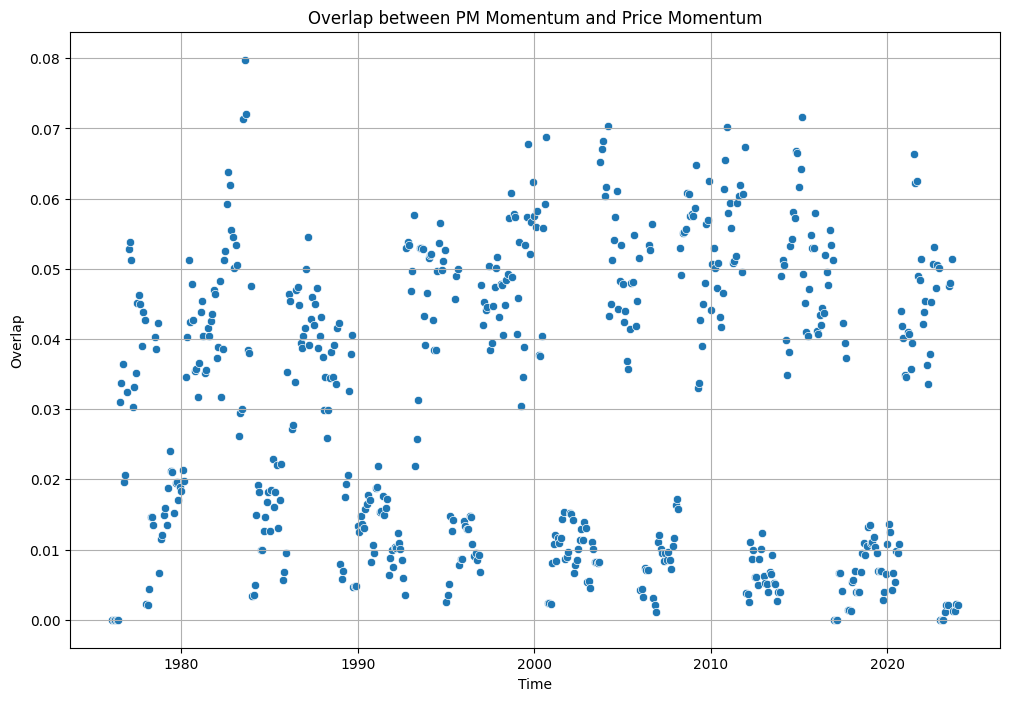
\includegraphics[width=.85\textwidth]{Images/pm_mom_overlap.png}
    \end{figure}
\end{frame}

\begin{frame}
    \frametitle{Conditional Strategy}
    \begin{block}{What can be improved?}
        We want to control the effect of price momentum while building long-short profit margin momentum portfolio. 
        We build long-short double sorted portfolios conditioning on PM momentum and price momentum. 
        We compared the following two long-short portfolios.
        \begin{itemize}
            \item High PM $\mid$ \text{High Price} $-$ \text{Low PM} $\mid$ \text{High Price}
            \item High PM $\mid$ \text{Low Price}  $-$ \text{Low PM} $\mid$ \text{Low Price}
        \end{itemize}
    \end{block}
\end{frame}

\begin{frame}{Conditional Strategy: Results}
    \begin{minipage}[c]{0.6\textwidth}
        \centering
        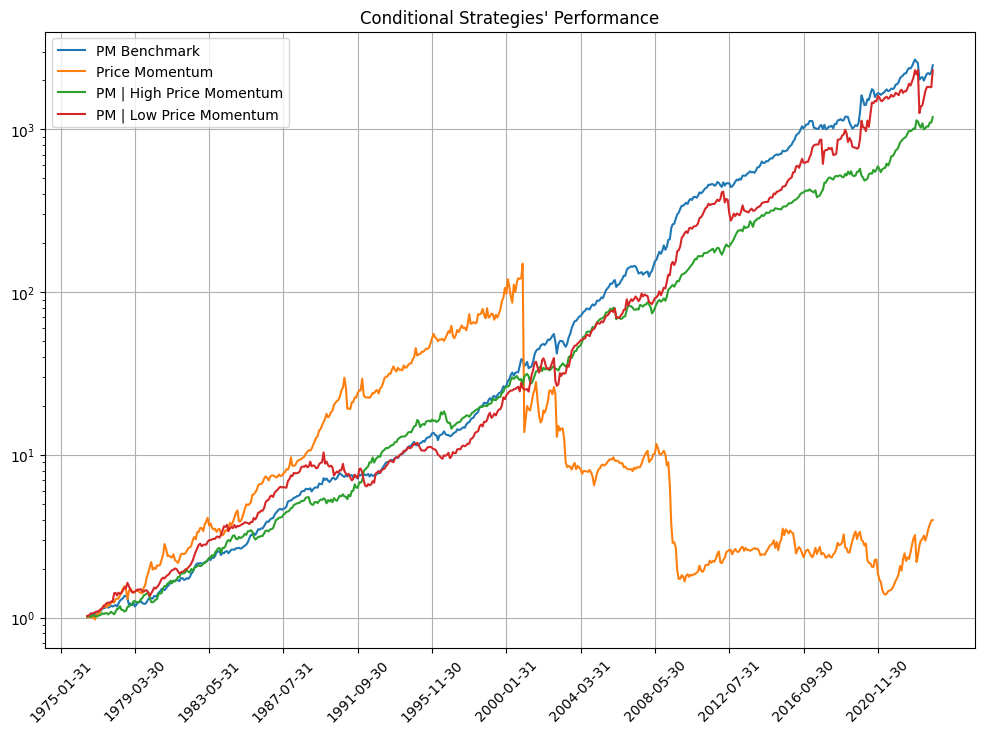
\includegraphics[width=\textwidth]{Images/condition.png}
    \end{minipage}
    \hspace{0.01\textwidth} 
    \begin{minipage}[c]{0.3\textwidth}
        \centering
        \scalebox{0.4}{
\begin{tabular}{lccc}
\toprule
      & PM Momentum & High Price M. & Low Price M. \\
\midrule
Mean & 17.34\% & 15.68\% & 18.43\% \\
Std & 12.55\% & 11.72\% & 19.60\% \\
SR & 1.38 & 1.34 & 0.94 \\
MDD & 25.70\% & 21.79\% & 45.56\% \\
\bottomrule
\end{tabular}
        }
    \end{minipage}
\end{frame}

\begin{frame}{Conditional Strategy: Results(Since 2010)}
    \begin{minipage}[c]{0.6\textwidth}
        \centering
        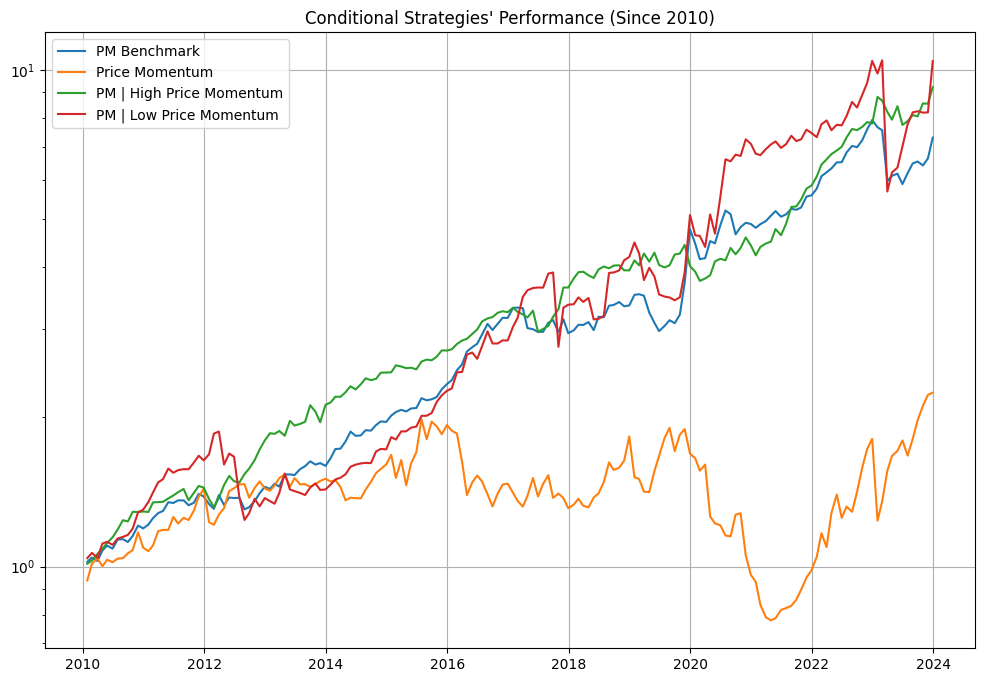
\includegraphics[width=\textwidth]{Images/condition_new.png}
    \end{minipage}
    \hspace{0.01\textwidth} 
    \begin{minipage}[c]{0.3\textwidth}
        \centering
        \scalebox{0.4}{
\begin{tabular}{lccc}
\toprule
& PM Benchmark & High Price PM. & Low Price PM. \\
\midrule
Mean & 15.39\% & 16.65\% & 20.59\% \\
Std & 15.03\% & 11.73\% & 26.25\% \\
SR & 1.02 & 1.42 & 0.78 \\
MDD & 25.70\% & 15.36\% & 45.56\% \\
\bottomrule
\end{tabular}
        }
    \end{minipage}
\end{frame}

\section{Conclusion}
\begin{frame}{Conclusion}
    \begin{itemize}
        \item Profit margin momentum strategy provides a more stable and significant performance compared with price momentum.
        \item The profit margin momentum strategy is not subsumed by the traditional Fama-French 3 factors and price momentum.
        \item Though the overlap of the profit margin momentum and price momentum strategies is relatively low, the conditional strategy generates a more stable performance
        by reducing the effect of price momentum.
    \end{itemize}
\end{frame}

\begin{frame}
    \centering
    {\Huge Thank You!}
\end{frame}
    
\end{document}